\chapter{Introduction}
\setcounter{page}{1}
\begin{quotation}
\noindent ``\emph{The question of whether a computer can think is no more 
	interesting than the question of whether a submarine can swim.}''
\begin{flushright}\textbf{Edsger W. Dijkstra}\end{flushright}
\end{quotation}

\vspace*{0.5cm}

\section{Context and goals}
One could trace back the birth of the machine learning idea to Alan Turing's 
seminal paper, \textit{Computing Machinery and Intelligence} 
\cite{turing1950computing}. Although the computer science context around his
work was only at its beginnings (at least compared to today), Turing already felt
the need to think of ways to transcend the fixed set of rules a computer had
to interpret and execute. As computer science grew, and as the field of
artificial intelligence went through its ebbs and flows throughout the years,
machine learning evolved from an idea to a prolific field of research, and
some of its topics saw massive application into real world domains.\\

The idea of machine learning evolved to become the design of computer systems
which perform tasks without having been explicitly programmed to perform them.
Instead of writing specific task-related rules, a machine learning practitioner
designs a model which will learn to perform correctly by experience, that is by
looking at examples of correct task completion, but also by making and looking
at mistakes.\\

The most popular and widely used machine learning algorithms and techniques
usually come from supervised and unsupervised machine learning.
The broad goal of supervised machine learning is to find a function that maps
some input vector $x$ to some output vector $y$. One example of this would be
to try to categorise patients that either have or don't have some disease. 
The input vector $x$ could contain measurements such as blood pressure, the 
quantity of a given substance in the patient's blood, etc. The output vector
$y$ would be either $[0]$ if the patient is ill, and $[1]$ if the patient is
not.\\

\begin{figure}
	\centering
	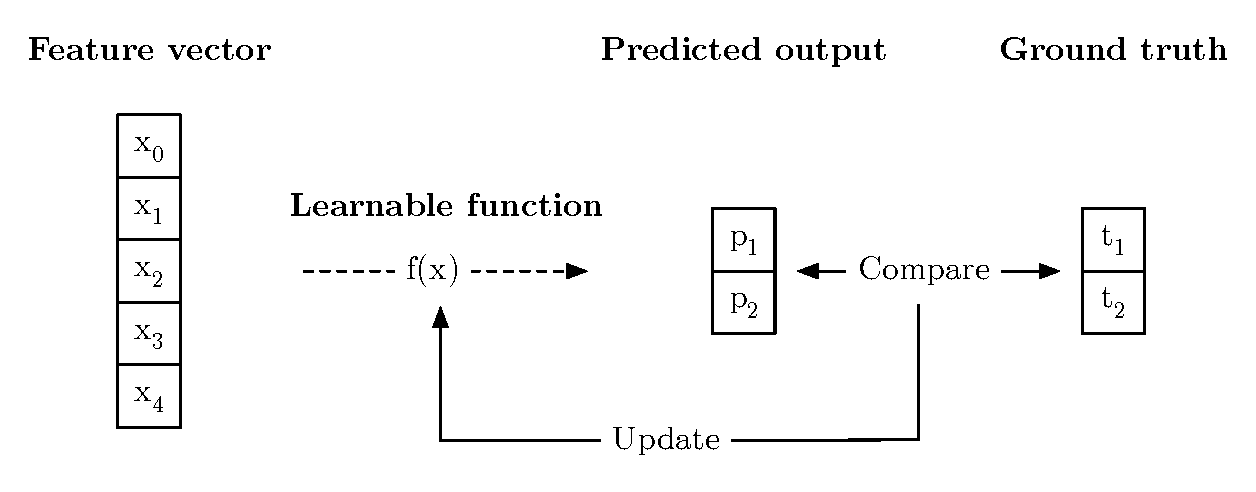
\includegraphics[width=0.8\linewidth]{fig/supervised_ml.eps}
	\caption{The supervised learning process. A feature vector and its ground
	truth $(x, t)$ are sampled from the training set. A learnable
	function computes a prediction based on the feature vector (which 
	contains measurements). We compare this prediction with the ground 
	truth and update the learnable function to minimise the error
	between the prediction and the ground truth, repeating the process
	until the function has reached a good enough accuracy.}
	\label{fig:supervised_ml}
\end{figure}

If we could find a function mapping $x$ to $y$, we could compute a probability
distribution over whether the patient is ill or not only by knowing $x$. 
Supervised machine learning provides the following general process (illustrated
in Figure~\ref{fig:supervised_ml}) to find
such a function : one defines a model which has
\textit{learnable parameters}; that is values which impact the output of the
function, and performs \textbf{training}. The process of training is to
sample data points from a \textbf{training set}, containing pairs of input
vectors and output vectors. We then feed the input vector to the model, compare
the output that we get from the model with the output we are supposed to get,
and tune the learnable parameters so to minimise the error between the model
output and the correct output. We repeat this process, showing many samples
of the training set to the model until it reaches a good enough accuracy. Once
the function is learned, we can predict to a certain level of accuracy new 
outputs from unseen feature vectors: for example, we can compute the probability
of a new patient being ill from his or her measurements.\\

Unsupervised learning, although different from supervised learning as the
training sets usually do not have output vectors, is more about finding
structure in the dataset; but we can assume for the sake of this point that
the process is largely the same : sample data, update learnable parameters
until the model is fixed at a good enough accuracy and inference can be
performed data point by data point after training.\\

To the experienced reader, unsupervised machine learning and supervised machine
learning might sound like fancy names for statistics; and one could argue that
they are indeed. A subfield of machine learning that veers off slightly more
from statistics and subjectively gets closer to human-like behaviour
would be \textbf{reinforcement learning}. In this setting, we train an agent
(an entity which can perform actions, that is anything that can perceive and
act: robots, simulated software agents, ...), 
which is situated in an environment, to perform actions that will maximise
a reward given by the environment. This endeavour is orders of magnitudes more
complex to handle at first glance. One has to train an agent that has to make
assumptions about the environment it is situated in, but also set up a
potentially hierarchical strategy involving several sequences of actions.\\

This process works by letting the agent interact with the environment for many
sessions, until it figures out what actions, and what sequences of actions lead
to high rewards. This is the training process of a reinforcement learning agent.
One example of this is the CartPole problem \cite{barto-cartpole} where the
agent controls a cart on which a pole is balanced (see
Figure~\ref{fig:cartpole_illustration}). The goal is to keep the
pole balanced for as long as possible by nudging the cart left or right. The
agent receives the position of the cart, the velocity of the cart, the pole
angle and the pole velocity at tip as a state observation from the environment,
and has to push the cart either left or right. The agent will first perform
randomly, but sooner or later, it will figure out how to balance the pole.\\

\begin{figure}
	\centering
	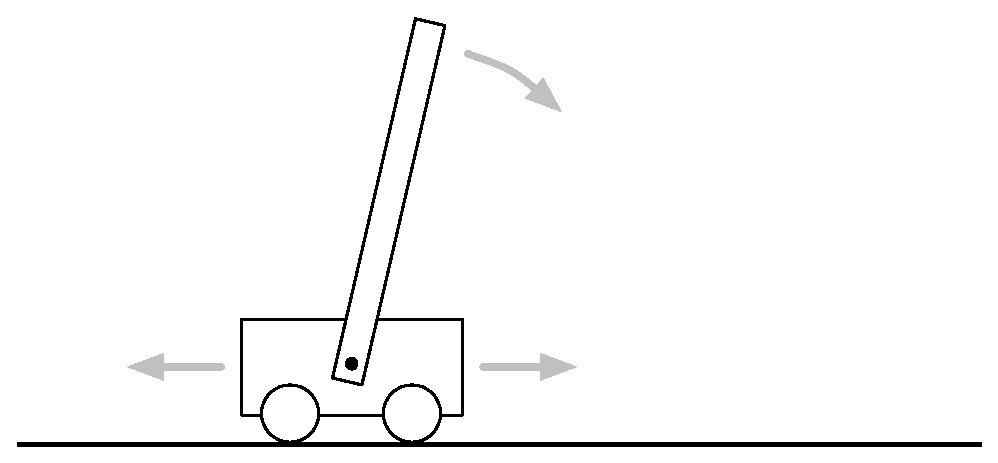
\includegraphics[width=0.8\linewidth]{fig/cartpole.eps}
	\caption{An illustration of the CartPole problem}
	\label{fig:cartpole_illustration}
\end{figure}

One common issue between all of the techniques described above is that once
training is over, the behaviour of the trained agent or model will not change
or adapt once the conditions, or some intrinsic parameters of the problem
change. If we present the CartPole agent with a pole that is twice as heavy,
or twice as long as the one it has been trained with, it will likely fail to 
balance the pole. We have taught an agent how to solve one task, but we have
not taught it to learn how to solve a task. This thesis will explore ways to 
teach an agent how to learn to solve tasks.



\section{Structure}
We will set the theoretical foundations needed to understand the methods used
in the experiments that will follow in part I. Reinforcement learning will
obviously be covered as well as artificial neural networks which serve as 
excellent learnable functions and have proven to work extremely well by
pushing the state of the art in many domains.\\

In part II, focus will be set on meta reinforcement learning : first we will
have to understand what it is and its goals are; then we will explore different
aspects and challenges related to it by inspecting how different experiments
and different parameters affect its performance.\\

Throughout part II, an analysis of the application of meta-learning to the
CartPole problem will be carried on, and discussion about why it performs
well in certain cases and why it fails in other cases will take place.


\section{Main contributions}
\noindent
Here are the main contributions
\vspace{1cm}
\begin{enumerate}
    \item hello
\end{enumerate}

\clearpage
\section{Notations}

%
notations, signification, page where it is defined and reference
\
